\subsubsection{UC13 - Effettua una prenotazione}
\begin{figure}[h]
	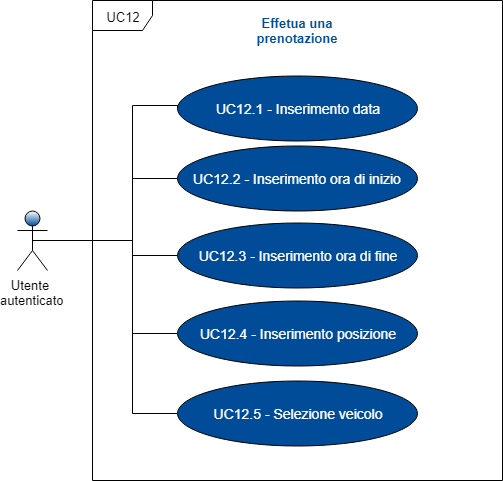
\includegraphics[width=10cm]{res/images/UC13Effettuaprenotazione.png}
	\centering
	\caption{UC13 - Effettua una prenotazione}
\end{figure}
\begin{itemize}
	\item \textbf{Attori Primari}: utente autenticato;
	\item \textbf{Descrizione}: l'utente può ricercare un veicolo sfruttando diversi parametri e prenotare quello più adatto alle sue esigenze.
	\item \textbf{Scenario principale}: l'utente per effettuare la prenotazione di un veicolo avrà a disposizione una maschera di ricerca che gli permetterà di filtrare i veicoli secondo questi parametri:
	\begin{itemize}
		\item data [UC13.1];
		\item ora di inizio [UC13.2];
		\item ora di fine [UC13.3];
		\item posizione [UC13.4]. 
	\end{itemize}
	l'utente avrà quindi a disposizione una lista e/o mappa di veicoli conformi alle sue preferenze di cui potrà visualizzare:
	\begin{itemize}		
		\item marca;
		\item modello;
		\item costo orario;
		\item immagine del veicolo.
	\end{itemize}
	Successivamente l'utente selezionerà il veicolo più consono alle sue necessità e potrà inviare la richiesta di prenotazione [UC13.5].
	\item \textbf{Precondizione}: l'applicazione rende disponibile il filtro per la ricerca;
	\item \textbf{Post-condizione}: il veicolo risulta prenotato correttamente.
\end{itemize} 
\subsubsection{UC13.1 - Inserimento data}
\begin{itemize}
	\item \textbf{Attori Primari}: utente autenticato;
	\item \textbf{Descrizione}: al fine di rendere il filtro di ricerca più stringente, l'utente può inserire in un apposito campo la data in cui intende prenotare il veicolo;
	\item \textbf{Scenario principale}: l'utente compila il campo relativo alla data;	
	\item \textbf{Precondizione}: l'applicazione ha reso disponibile il campo per l'inserimento della data;
	\item \textbf{Postcondizione}: l'utente ha compilato il campo con la data in cui intende prenotare un veicolo.	
\end{itemize}
\subsubsection{UC13.2 - Inserimento ora di inizio}
\begin{itemize}
	\item \textbf{Attori Primari}: utente autenticato;
	\item \textbf{Descrizione}: al fine di rendere il filtro di ricerca più stringente, l'utente può inserire in un apposito campo l'ora di inizio in cui s'intende prenotare il veicolo;
	\item \textbf{Scenario principale}: l'utente compila il campo relativo all'ora di inizio;	
	\item \textbf{Precondizione}: l'applicazione ha reso disponibile il campo per l'inserimento dell'ora di inizio;
	\item \textbf{Postcondizione}: l'utente ha compilato il campo con l'ora di inizio in cui intende prenotare un veicolo.	
\end{itemize}
\subsubsection{UC13.3 - Inserimento ora di fine}
\begin{itemize}
	\item \textbf{Attori Primari}: utente autenticato;
	\item \textbf{Descrizione}: al fine di rendere il filtro di ricerca più stringente, l'utente può inserire in un apposito campo l'ora di fine in cui s'intende prenotare il veicolo;
	\item \textbf{Scenario principale}: l'utente compila il campo relativo all'ora di fine;	
	\item \textbf{Precondizione}: l'applicazione ha reso disponibile il campo per l'inserimento dell'ora di fine;
	\item \textbf{Postcondizione}: l'utente ha compilato il campo con l'ora di fine in cui intende prenotare un veicolo.	
\end{itemize}
\subsubsection{UC13.4 - Inserimento posizione}
\begin{itemize}
	\item \textbf{Attori Primari}: utente autenticato;
	\item \textbf{Descrizione}: al fine di rendere il filtro di ricerca più stringente, l'utente può inserire in un apposito campo la posizione in cui si trova per poter cercare intorno a se i veicoli;
	\item \textbf{Scenario principale}: l'utente compila il campo relativo alla posizione;	
	\item \textbf{Precondizione}: l'applicazione ha reso disponibile il campo per l'inserimento della posizione;
	\item \textbf{Postcondizione}: l'utente ha compilato il campo con la posizione.	
\end{itemize}
\subsubsection{UC13.5 - Selezione veicolo}
\begin{itemize}
	\item \textbf{Attori Primari}: utente autenticato;
	\item \textbf{Descrizione}: una volta filtrati i veicoli, l'utente potrà scegliere quello più di suo gradimento, selezionarlo e prenotarlo tramite l'apposito pulsante;
	\item \textbf{Scenario principale}: 
	l'utente, dopo aver filtrato i veicoli, viene portato nella sezione "lista veicoli". In questa sezione verranno mostrati i veicoli filtrati sotto forma di lista in cui l'utente potrà selezionare un veicolo e prenotarlo con l'apposito pulsante;
	\item \textbf{Scenario alternativo}: l'utente, dopo aver filtrato i veicoli, cambia ed entra nella sezione "mappa". In questa sezione verranno mostrati i veicoli filtrati sotto forma di mappa in cui l'utente potrà selezionare un veicolo intorno al punto, che è la sua posizione, e prenotarlo con l'apposito pulsante;
	\item \textbf{Precondizione}: l'applicazione ha reso disponibile all'utente almeno un veicolo selezionabile;
	\item \textbf{Postcondizione}: l'utente ha prenotato correttamente il veicolo.
\end{itemize}

